\documentclass[journal,twocolumn,12pt]{ieeesyscoin}
\usepackage{cite}
\usepackage{amsmath,amssymb,amsfonts}
\usepackage{algorithmic}
\usepackage{enumitem}
\usepackage{caption}
\usepackage{xcolor}
\usepackage{graphicx}
\usepackage{textcomp}
\usepackage{multirow}
\usepackage{lipsum}
\usepackage[switch]{lineno}
\def\BibTeX{{\rm B\kern-.05em{\sc i\kern-.025em b}\kern-.08em
    T\kern-.1667em\lower.7ex\hbox{E}\kern-.125emX}}
\begin{document}
\linenumbers
\history{}

\title{\centering DAOSYS: An Autonomous Service Engine for Decentralized Finance}
\author{\centering  \uppercase{Cyotee Doge}\authorrefmark{1}, 
\uppercase{Ian C. Moore, PhD}\authorrefmark{2},
\uppercase{Ryland Arbour}\authorrefmark{3}, and
\uppercase{Jagdeep Sidhu, MSc}\authorrefmark{4}}

\address[1]{\centering DAO Advisor, Syscoin Platform (e-mail: cyotee@syscoin.org)}
\address[2]{\centering  Syscoin Researcher, Syscoin Platform (e-mail: imoore@syscoin.org)}
\address[3]{\centering  L2 Advisor, Syscoin Platform (e-mail: rylandarbour@syscoin.com)}
\address[4]{\centering Syscoin Lead Developer, (e-mail: sidhujag@syscoin.org)}
\tfootnote{}

\markboth
{Cyotee \headeretal: DAOSYS: An Autonomous Service Engine for Decentralized Finance}
{Cyotee \headeretal: DAOSYS: An Autonomous Service Engine for Decentralized Finance}

\corresp{}

\begin{abstract}
Despite popular perception, treasuries of Dentralized Autonomous Organizations (DAOs) tend to be centrally controlled and do not fully reflect the ethos of cryptocurrency (i.e., \textit{not your keys, not your coins}). DAOSYS solves this problem with its new Autonomous Service Engine (ASE) technology by deploying a reference platform for self-sovereign capital coordination. This is made possible by further innovating on the multi-faceted proxy standards defined in EIP-2535. The ASE will serve as the cornerstone of all SYS Labs decentralized finance (DeFi) products, as supported by the Syscoin Platform.
\end{abstract}

\begin{keywords}
DAOSYS, Decentralized Autonomous Organization, Decentralized Finance, SYS Labs, EIP-2535
\end{keywords}

\titlepgskip=-15pt

\maketitle

\section{Introduction}
\label{sec:introduction}

The objective of a decentralized autonomous organization (DAO) is to solve the principal-agent dilemma. This dilemma is a result of misaligned incentives where agents acting in a system are incentivized towards their own benefit over the benefit of a principle or other agents acting within the system \cite{San83}. Typically, these are found in centralized systems where the central acting authority is the main compromised agent. The DAO solves this by decentralizing the governance process by utilizing smart contracts running on open source blockchains.

The first inception of the DAO concept happened in May 2016 out of the Ethereum community, which was known as Genesis DAO, and was built as a smart contract on the Ethereum blockchain. However, this resulted in the well known DAO Hack which resulted in the draining of \$60M USD worth of funds from its treasury \cite{Sie22}. Today, there are many DAOs in operation with Uniswap, Aave and Maker DAO being amongst the most popular. However, these DAOs still fundamentally violate the core value proposition of self sovereignty that crypto currency promises, where DAOs currently take ownership of capital managed in a treasury controlled by a few individuals. This is the problem that DAOSYS intends to address.

DAOSYS vision is to operate like a pure automated market maker (AMM) and be implemented in a manner that does not require external controls. It addresses this core issue via its new Autonomous Service Engine (ASE) technology \cite{Sys22}, hence allowing DAOs to be more autonomous and fully decentralized. One of the interesting by-products of this technology will allow users to test, implement and realize countless decentralized finance (DeFi) usecase designs.

\section{Governance}
\label{sec:governance}

One of the distinguishing features of a DOA is the fact that it is a governance structure for a group of people to make decisions. Unlike traditional organizations (e.g., private companies, non-governmental organizations, charities, etc.) which have a centralized structure, these decisions are coordinated and enforced on a blockchain in a decentralized manner. 

DAOSYS has no top level governance. Applying the AMM model to DAOs means that users create their own treasuries for specific ventures. These treasuries may apply a variety of governance solutions along with their treasuries. This allows for a compartmentalization of the politics that arise with any governance solution from the actual treasury management.

\begin{figure}[h!]
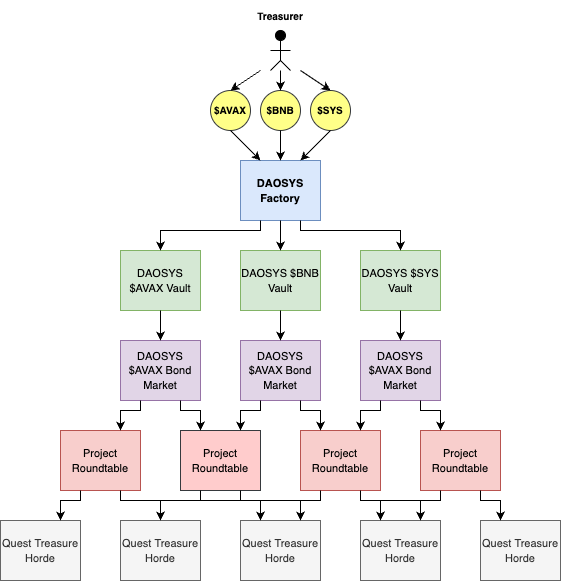
\includegraphics[width=3in]{img/governance.png}
\caption{DAOSYS Governance Structure} 
\label{fig:current_vs_zdag}
\end{figure} 

Under this model, the Syscoin Foundation behaves more like a software vendor. The factory makes open-source reference implementations of defi components available to compose into treasuries. Updates to these smart-contracts are available for deploying new pools that may be added to a DAO. This removes the need for a top-level governance solution that decides whether to include an update because users are free to create new pools.

A user creates a DAO by selecting which vaults and bond markets they would like to include. These vaults may come from four sources.

\subsection{Reuse an existing vault}

This works best for when users wish to maintain their position in one DAO, but want to add more pools to form a new DAO.

\subsection{Recreate an existing vault}

If it’s not broke, don’t fix it. The investment strategy implemented in a vault can be used across several instances of vault pools. This works well for new DAOs that wish to replicate the financial strategies of an existing DAO. Also for when the new DAO would like to invest in other DAOs using the same strategy.


\subsection{New pool with new investment strategy}

A user may wish to create a new DAO reusing functionality available from the factory, but configured in a novel manner. The flexibility available in the ASE means that even a simple strategy has several configuration options. This is useful for when a DAO wishes to adopt a novel investment strategy that might not have been previously viable.

\subsection{New pool with custom code}

The Syscoin Foundation makes internal decisions regarding what smart-contracts are available through the factory similar to open source software development. Because this only concerns the software available from the foundation, this does not need to be open to public governance. When the community at large wishes to release custom code outside the foundation, a user may use the factory to deploy their own factory offering their custom code. This new factory inherits the offerings of the parent factory and may add their own modules.

These pools form the foundation of the DAO. Autonomous and permissionless liquidity pools that act as the agreed upon foundation for DAO treasury management. From there users may launch further liquidity pools that may accept the DAOs Treasury Token for deposit. These form the Roundtables for managing ventures within the DAO. The Roundtables compartmentalize management teams, Councilors, of the various ventures being executed under a DAO’s mission statement. A Roundtable typically does not have it’s own governance token, instead using a Council Token used to resolve disputes by executing buyout options.

From the Roundtables, any Councilor may use their contribution to the Roundtable to launch a bond offering for a Quest. Quests define the bounty award and terms for completing a task. The Councilor that issues the quest puts their share of the treasury in escrow to fund the Quest. The interest being earned from that underlying position is then split to fund the bounty, compound into that position, and to sell on the bond market. This ensures that Questors know the payment for work they deliver is secured. And protects the Councilor from failure to deliver.

\section{Architecture}
\label{sec:architecture}

\lipsum[2-4]

\section{Tokenomics}
\label{sec:tokenomics}

\lipsum[1]

\subsection{Simulator}

\lipsum[2-4]

\section{RoadMap}
\label{sec:roadmap}

\subsection{SYSLabs}

\lipsum[1]

\subsection{L2: NEVM}

\lipsum[1]

\subsection{First Use Case: Masternode Yield Farming}

\lipsum[1]

\section{Summary}
\label{section:summary}
\lipsum[1]

\appendices

\section{EIP-2535 (Diamonds)}

\lipsum[1]

\begin{thebibliography}{00}

\bibitem{San83} S.J. Grossman, O.D. Hart, \textit{An Analysis of the Principal-Agent Problem}, Econometrica, Volume 51, Issue 1 (Jan., 1983), 7-46.

\bibitem{Sie22} D. Siegel, \textit{Understanding The DAO Attack}, Coindesk, Aug. 2022. Accessed on: Sept 2022. [Online]. Available: https://www.coindesk.com/learn/2016/06/25/understanding-the-dao-attack/

\bibitem{Sys22} Syscoin Dev Team, \textit{DAOSYS Lite Paper}, Accessed on: Sept 2022.  [Online]. Available:  https://github.com/syscoin/daosys

\bibitem{Sig21} J. Sidhu and I.C. Moore, \textit{Syscoin 4.0: A Peer-to-Peer Electronic Cash System Built For Business Applications}, Dec 2021, Accessed on: Sep 2022.  [Online]. Available:  https://syscoin.org/file/syscoin4-whitepaper.pdf

\end{thebibliography}


\EOD

\end{document}
